\documentclass{standalone}
\usepackage{tikz}

\begin{document}
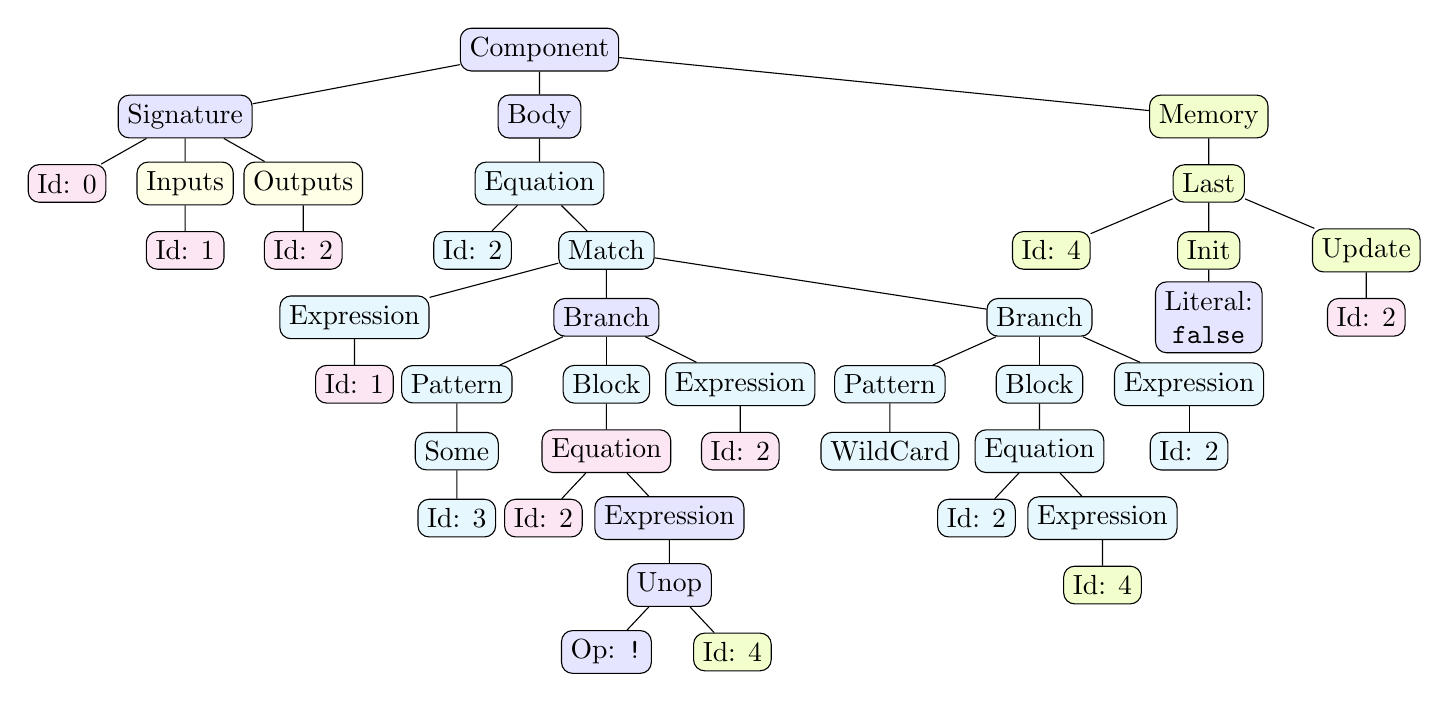
\begin{tikzpicture}[
                level distance=0.85cm, sibling distance=3cm,
                treenode/.style = {rectangle, rounded corners, draw, fill=blue!10, align=center}
        ]
        \node[treenode] {Component}
        child [sibling distance=4.5cm] { node[treenode] {Signature}
                        child [sibling distance=1.5cm] { node[treenode, fill=magenta!10] {Id: 0} }
                        child [sibling distance=1.5cm] { node[treenode, fill=yellow!10] {Inputs}
                                        child { node[treenode, fill=magenta!10] {Id: 1} }
                                }
                        child [sibling distance=1.5cm] { node[treenode, fill=yellow!10] {Outputs}
                                        child { node[treenode, fill=magenta!10] {Id: 2} }
                                }
                }
        child [sibling distance=4.5cm] { node[treenode] {Body}
                        child [sibling distance=4.5cm] { node[treenode, fill=cyan!10] {Equation}
                                        child [sibling distance=1.7cm] { node[treenode, fill=cyan!10] {Id: 2} }
                                        child [sibling distance=1.7cm] { node[treenode, fill=cyan!10] {Match}
                                                        child [sibling distance=3.2cm] { node[treenode, fill=cyan!10] {Expression} child { node[treenode, fill=magenta!10] {Id: 1} } }
                                                        child [sibling distance=3.2cm] { node[treenode] {Branch}
                                                                        child [sibling distance=1.9cm] { node[treenode, fill=cyan!10] {Pattern} child [sibling distance=3cm] { node[treenode, fill=cyan!10] {Some} child { node[treenode, fill=cyan!10] {Id: 3} } } }
                                                                        child [sibling distance=1.9cm] { node[treenode, fill=cyan!10] {Block}
                                                                                        child [sibling distance=3cm] { node[treenode, fill=magenta!10] {Equation}
                                                                                                        child [sibling distance=1.6cm] { node[treenode, fill=magenta!10] {Id: 2} }
                                                                                                        child [sibling distance=1.6cm] { node[treenode] {Expression}
                                                                                                                        child { node[treenode] {Unop}
                                                                                                                                        child { node[treenode] {Op: \texttt{!}} }
                                                                                                                                        child { node[treenode, fill=lime!20] {Id: 4} }
                                                                                                                                }
                                                                                                                }
                                                                                                }
                                                                                }
                                                                        child [sibling distance=1.7cm] { node[treenode, fill=cyan!10] {Expression} child { node[treenode, fill=magenta!10] {Id: 2} } }
                                                                }
                                                        child [sibling distance=5.5cm] { node[treenode, fill=cyan!10] {Branch}
                                                                        child [sibling distance=1.9cm] { node[treenode, fill=cyan!10] {Pattern} child [sibling distance=3cm] { node[treenode, fill=cyan!10] {WildCard} } }
                                                                        child [sibling distance=1.9cm] { node[treenode, fill=cyan!10] {Block}
                                                                                        child [sibling distance=3cm] { node[treenode, fill=cyan!10] {Equation}
                                                                                                        child [sibling distance=1.6cm] { node[treenode, fill=cyan!10] {Id: 2} }
                                                                                                        child [sibling distance=1.6cm] { node[treenode, fill=cyan!10] {Expression}
                                                                                                                        child { node[treenode, fill=lime!20] {Id: 4} }
                                                                                                                }
                                                                                                }
                                                                                }
                                                                        child [sibling distance=1.9cm] { node[treenode, fill=cyan!10] {Expression} child { node[treenode, fill=cyan!10] {Id: 2} } }
                                                                }
                                                }
                                }
                }
        child [sibling distance=8.5cm] { node[treenode, fill=lime!20] {Memory}
                        child [sibling distance=2cm] { node[treenode, fill=lime!20] {Last}
                                        child { node[treenode, fill=lime!20] {Id: 4} }
                                        child { node[treenode, fill=lime!20] {Init} child { node[treenode] {Literal:\\\texttt{false}} } }
                                        child { node[treenode, fill=lime!20] {Update} child { node[treenode, fill=magenta!10] {Id: 2} } }
                                }
                };
\end{tikzpicture}
\end{document}
